\section{Diagramas de secuencia de la Iteración I}

\par A lo largo de esta sección se muestran los diagramas de secuencia de los casos de uso de la iteración I. Cabe decir, que para cada diagrama de secuencia se sobreentiende que el coche debe estar arrancado y los subsistemas a utilizar deben estar activados.

\par El diagrama de secuencia  en la figura \ref{img:notif_velocidad_max} hace referencia al \nameref{tab:CDUE-05}. Se muestra el \textit{flujo de ejecución normal} en el que el sistema es capaz de interpretar las señales en la primera parte del cuadro \textit{alt} de la figura. La segunda parte del cuadro \textit{alt} muestra el \textit{flujo de ejecución alternativo} en el que la velocidad máxima se comprueba gracias a la posición GPS.

\begin{figure}[h]
  \begin{center}
    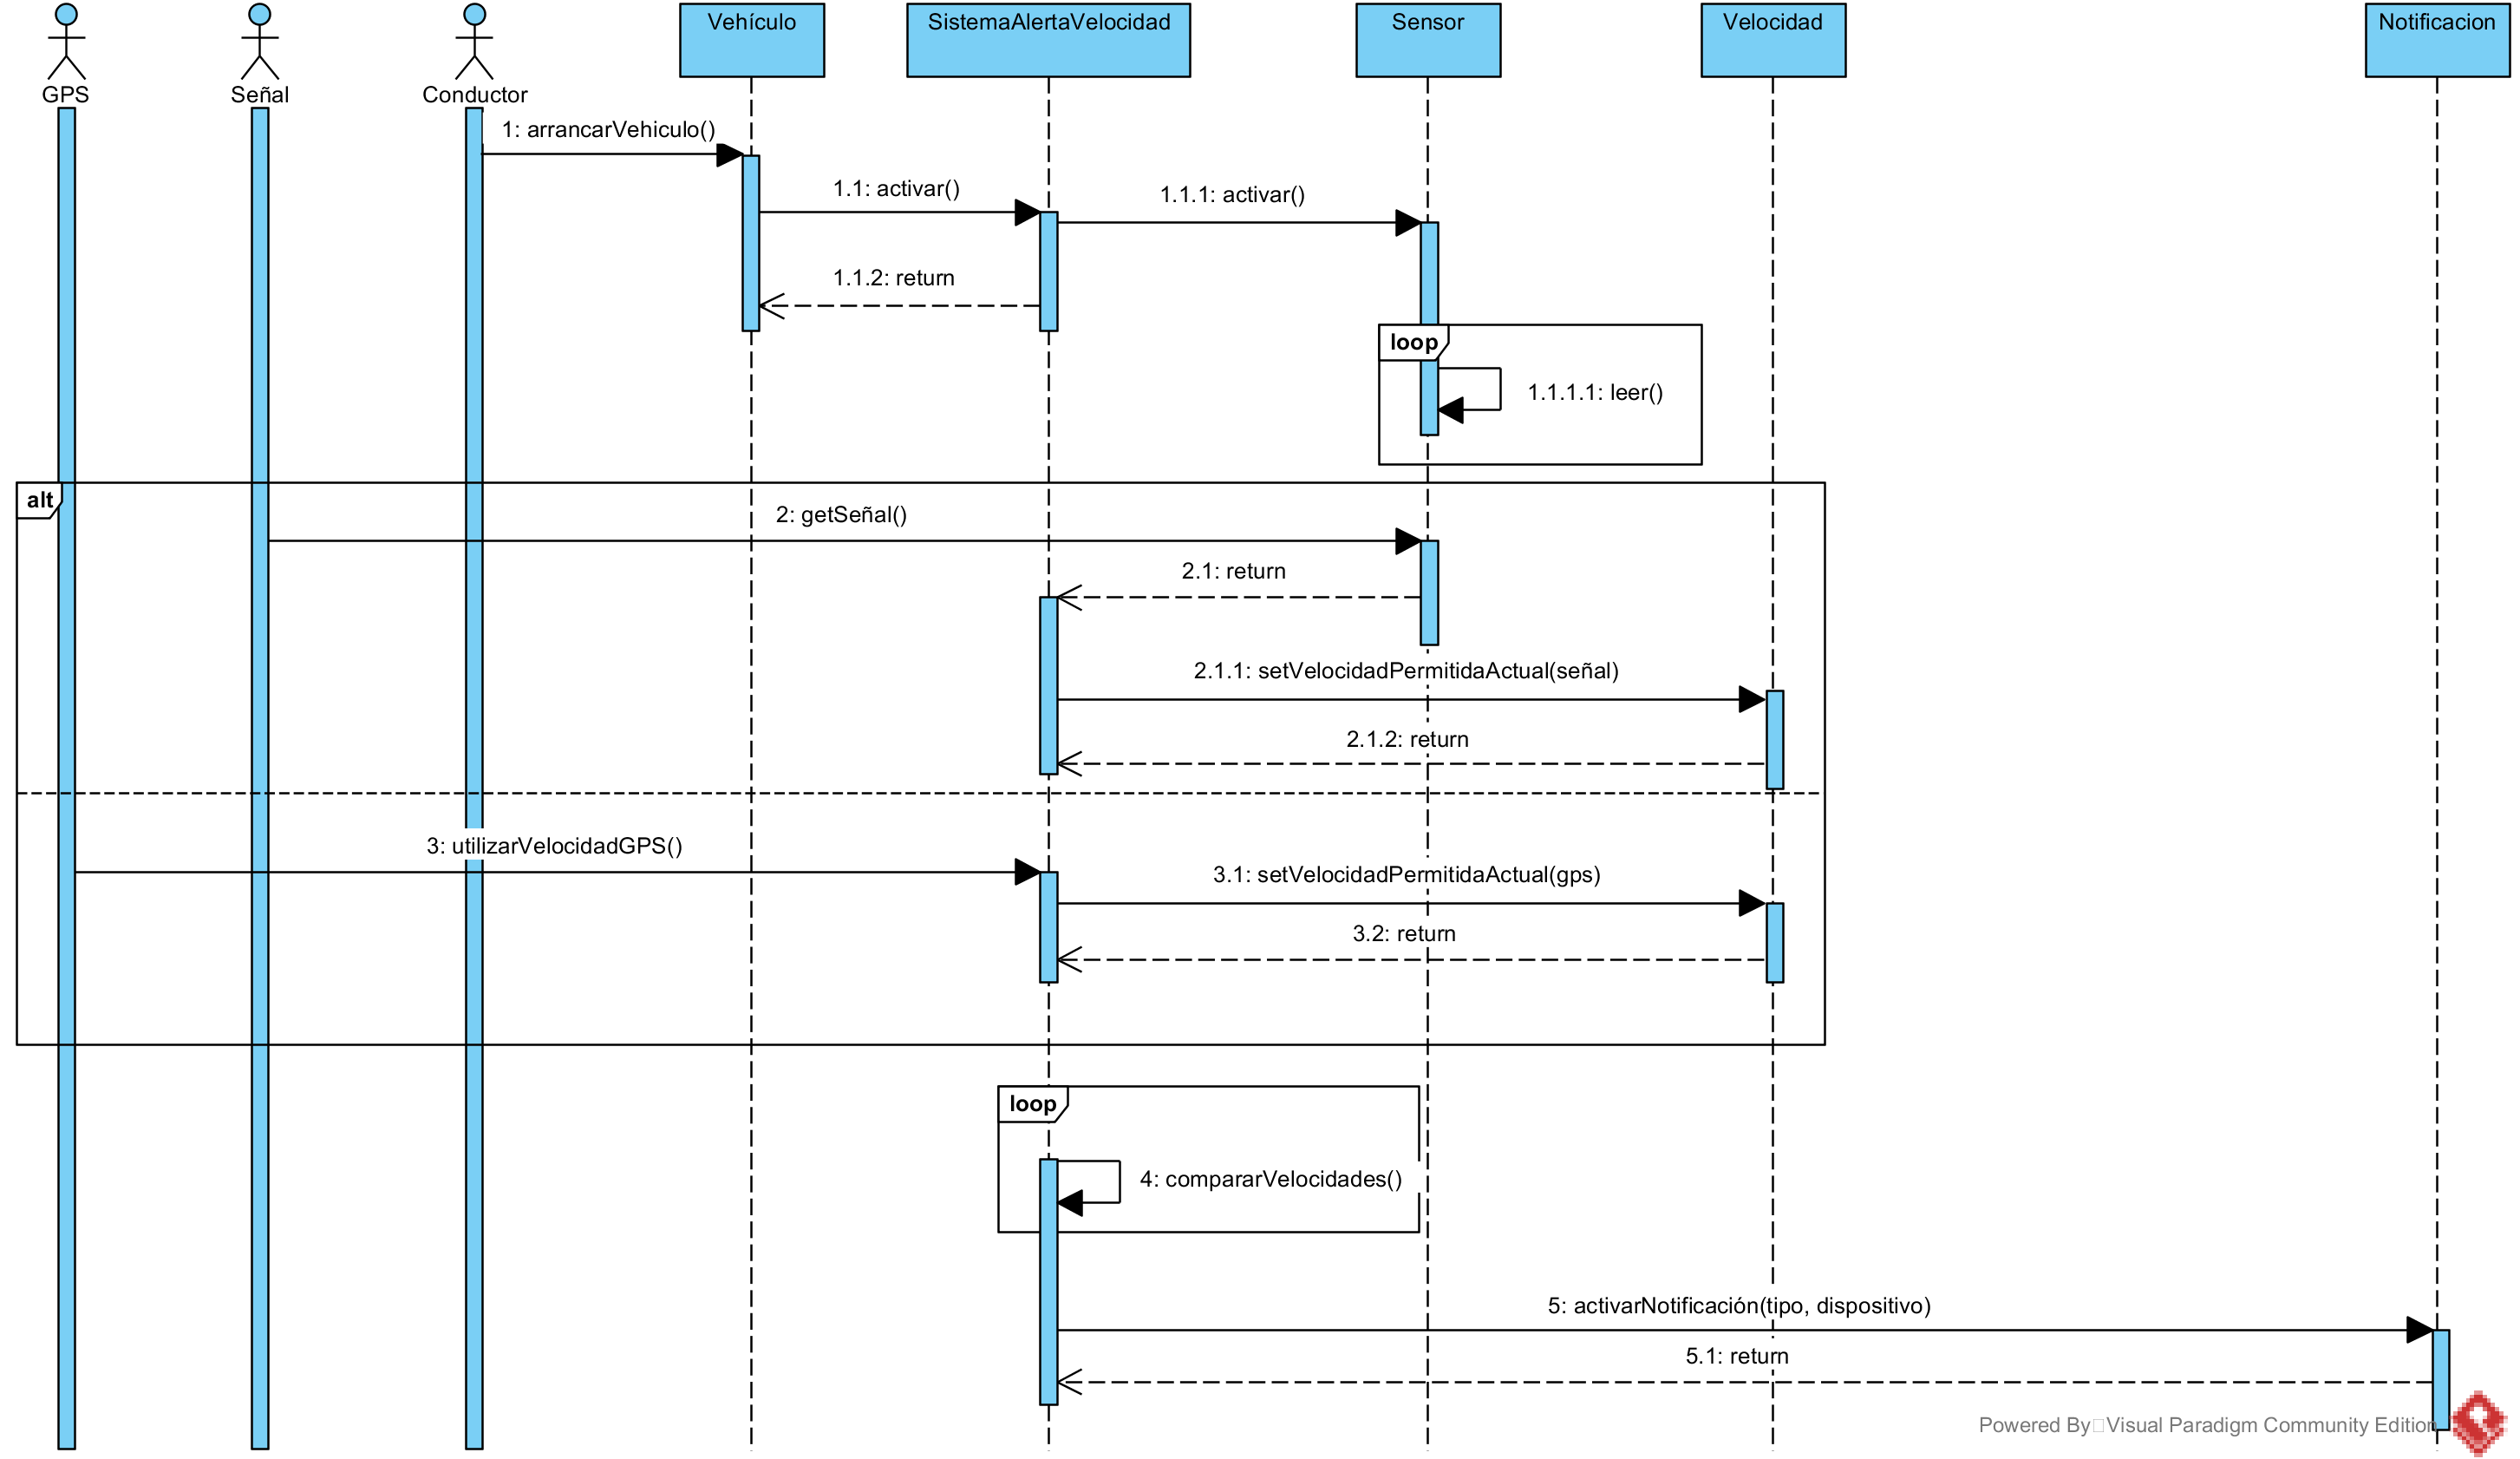
\includegraphics[width=0.8\textwidth]{./img/diagramas_de_secuencia/CDUE-05.png}
  \end{center}
  \caption{Diagrama de secuencia para el CDUE-05: \textit{Activar notificación por velocidad máxima}}
  \label{img:notif_velocidad_max}
\end{figure}

\clearpage

\par El diagrama de secuencia de la figura \ref{img:prep_vehiculo_impacto} hace referencia al \nameref{tab_CDUE-12}. En el \textit{flujo de ejecución normal} no se realiza ninguna acción, únicamente se comprueba si hay algún obstáculo en la carretera, pero como no se encuentra no se produce ninguna acción. En cambio, en el \textit{flujo de ejecución alternativo}, si que hay algún objeto en la calzada por lo que se desencadenan las acciones reflejadas en la figura.

\begin{figure}[h]
  \begin{center}
    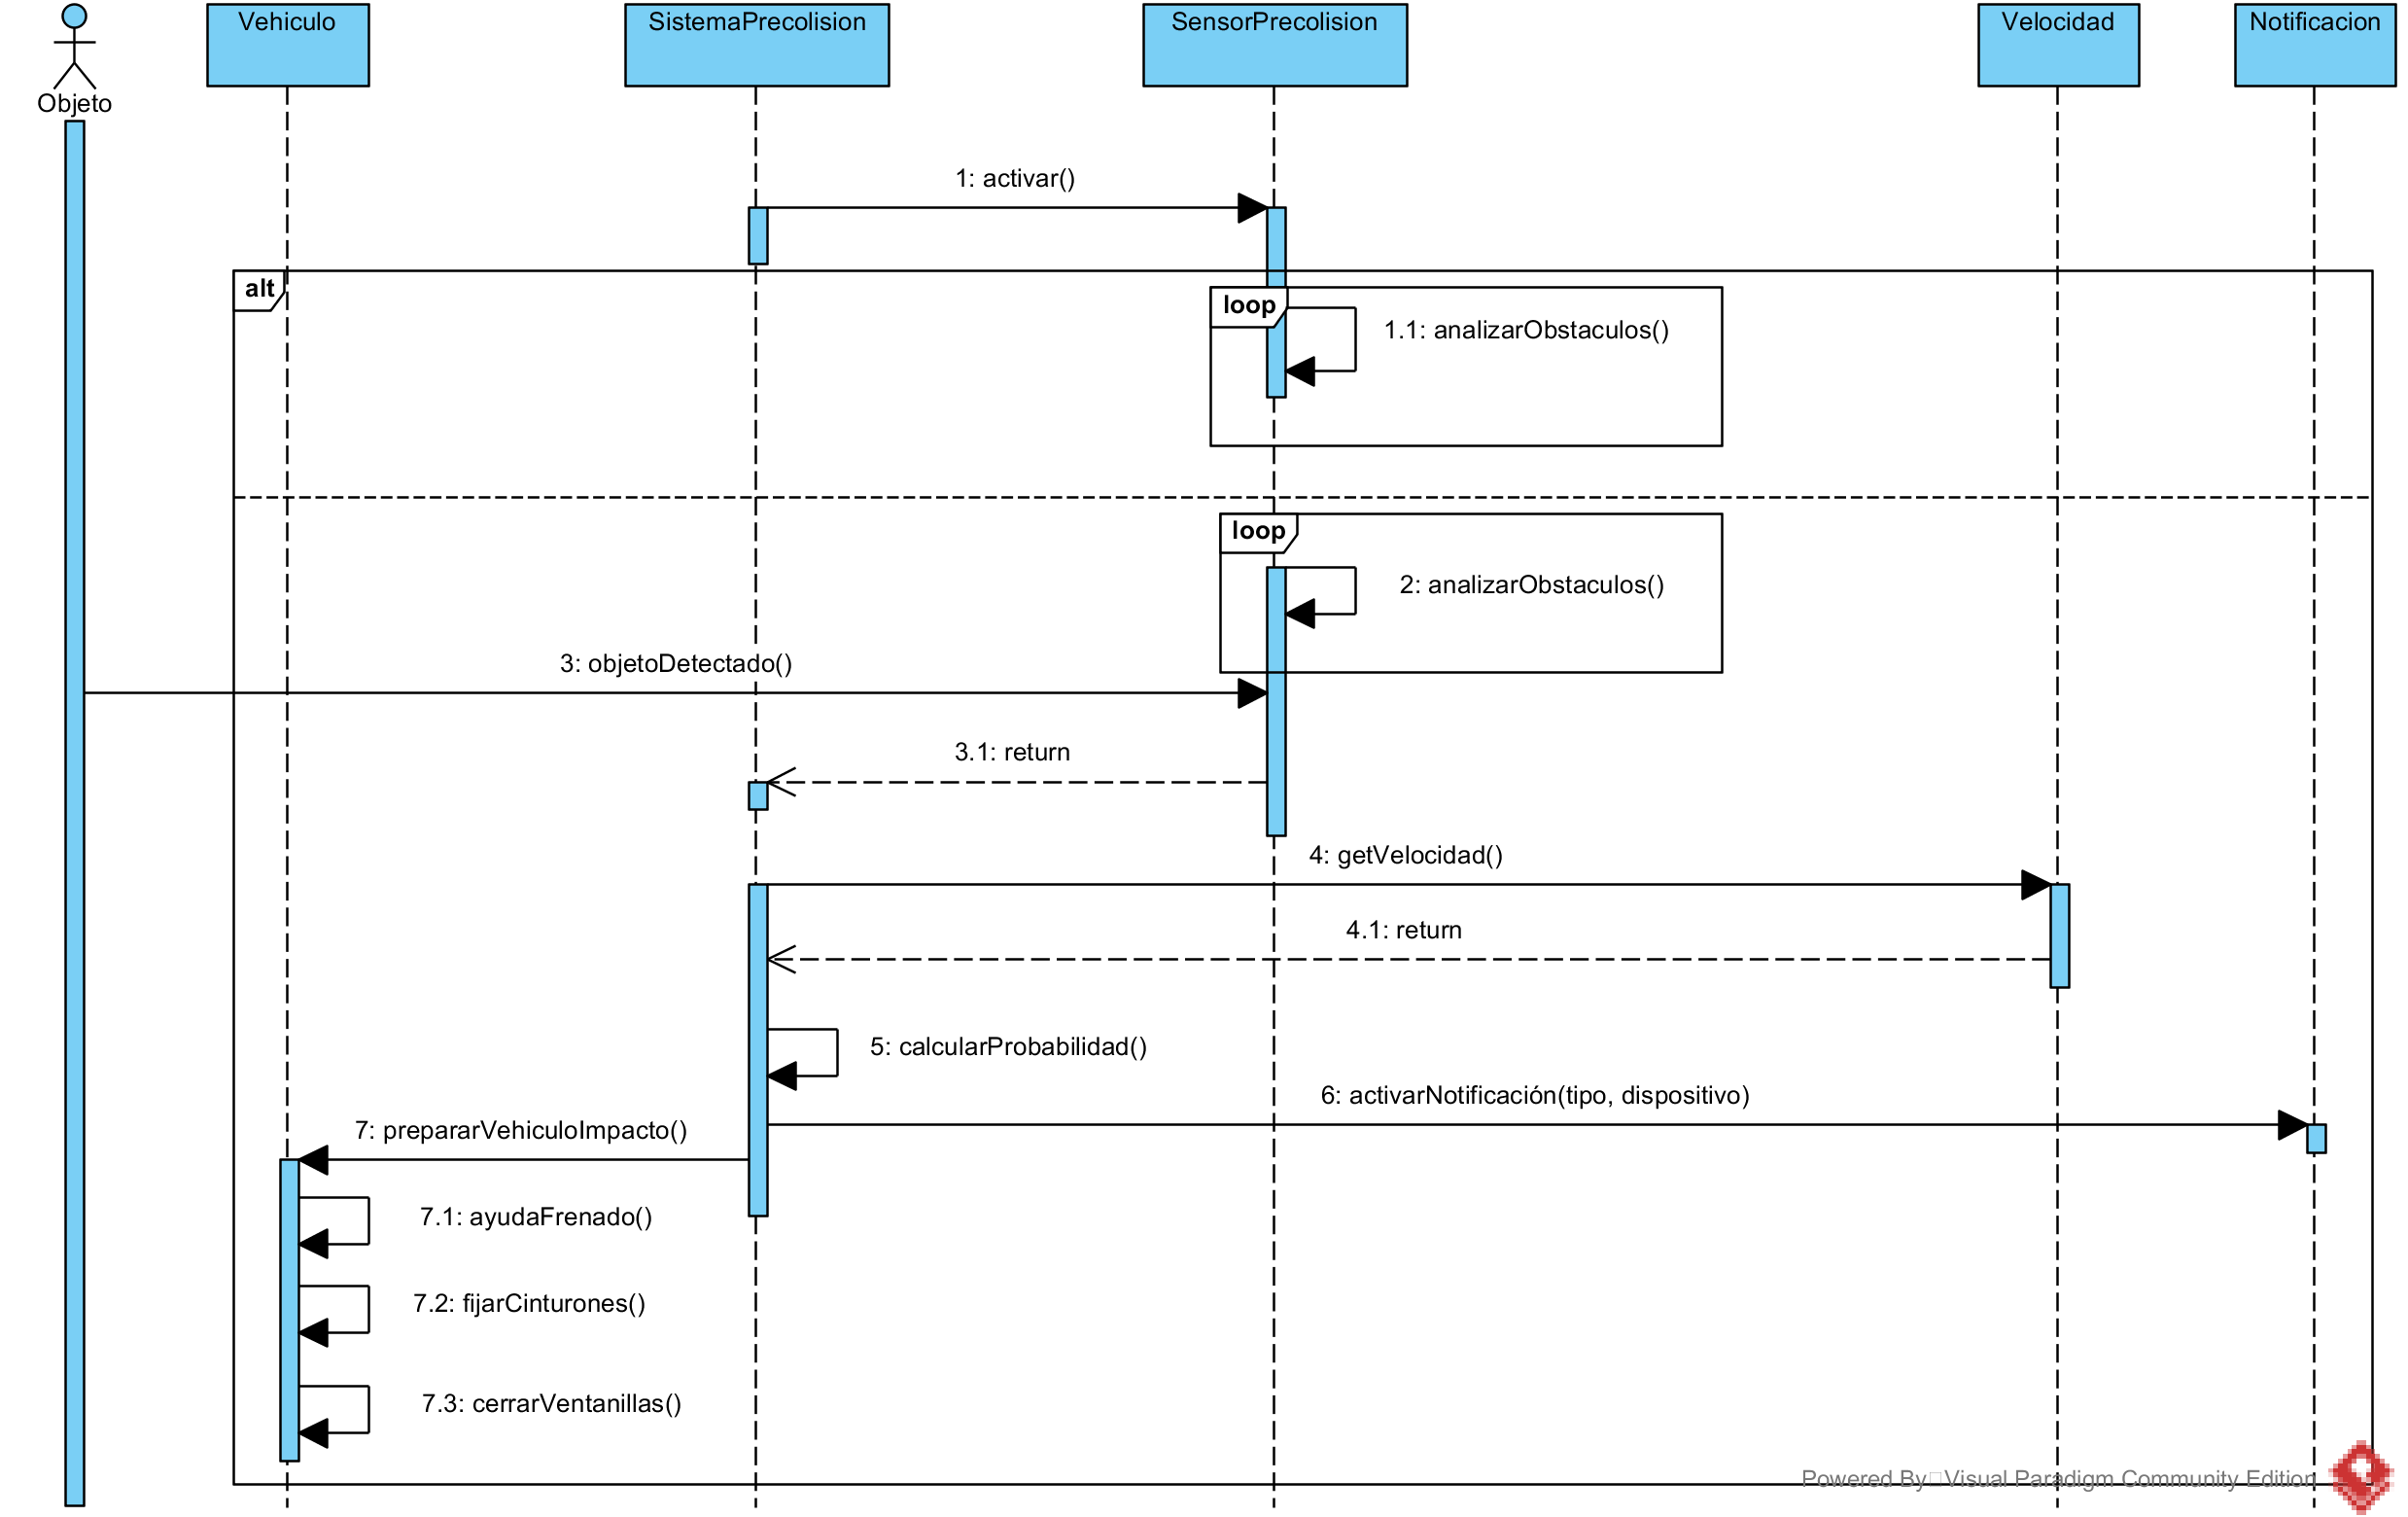
\includegraphics[width=0.8\textwidth]{./img/diagramas_de_secuencia/CDUE-12.png}
  \end{center}
  \caption{Diagrama de secuencia para el CDUE-12: \textit{Preparar vehículo para impacto}}
  \label{img:prep_vehiculo_impacto}
\end{figure}

\par El diagrama de secuencia de la figura \ref{img:not_riesgo_colision} hace referencia al \nameref{tab:CDUE-11}. Este diagrama es muy similar al de la figura \ref{img:prep_vehiculo_impacto}, lo que ocurre es que después de calcular la probabilidad en el \textit{flujo de ejecución alternativo} se activa una notificación en lugar de preparar el vehículo para el impacto.

\begin{figure}[h]
  \begin{center}
    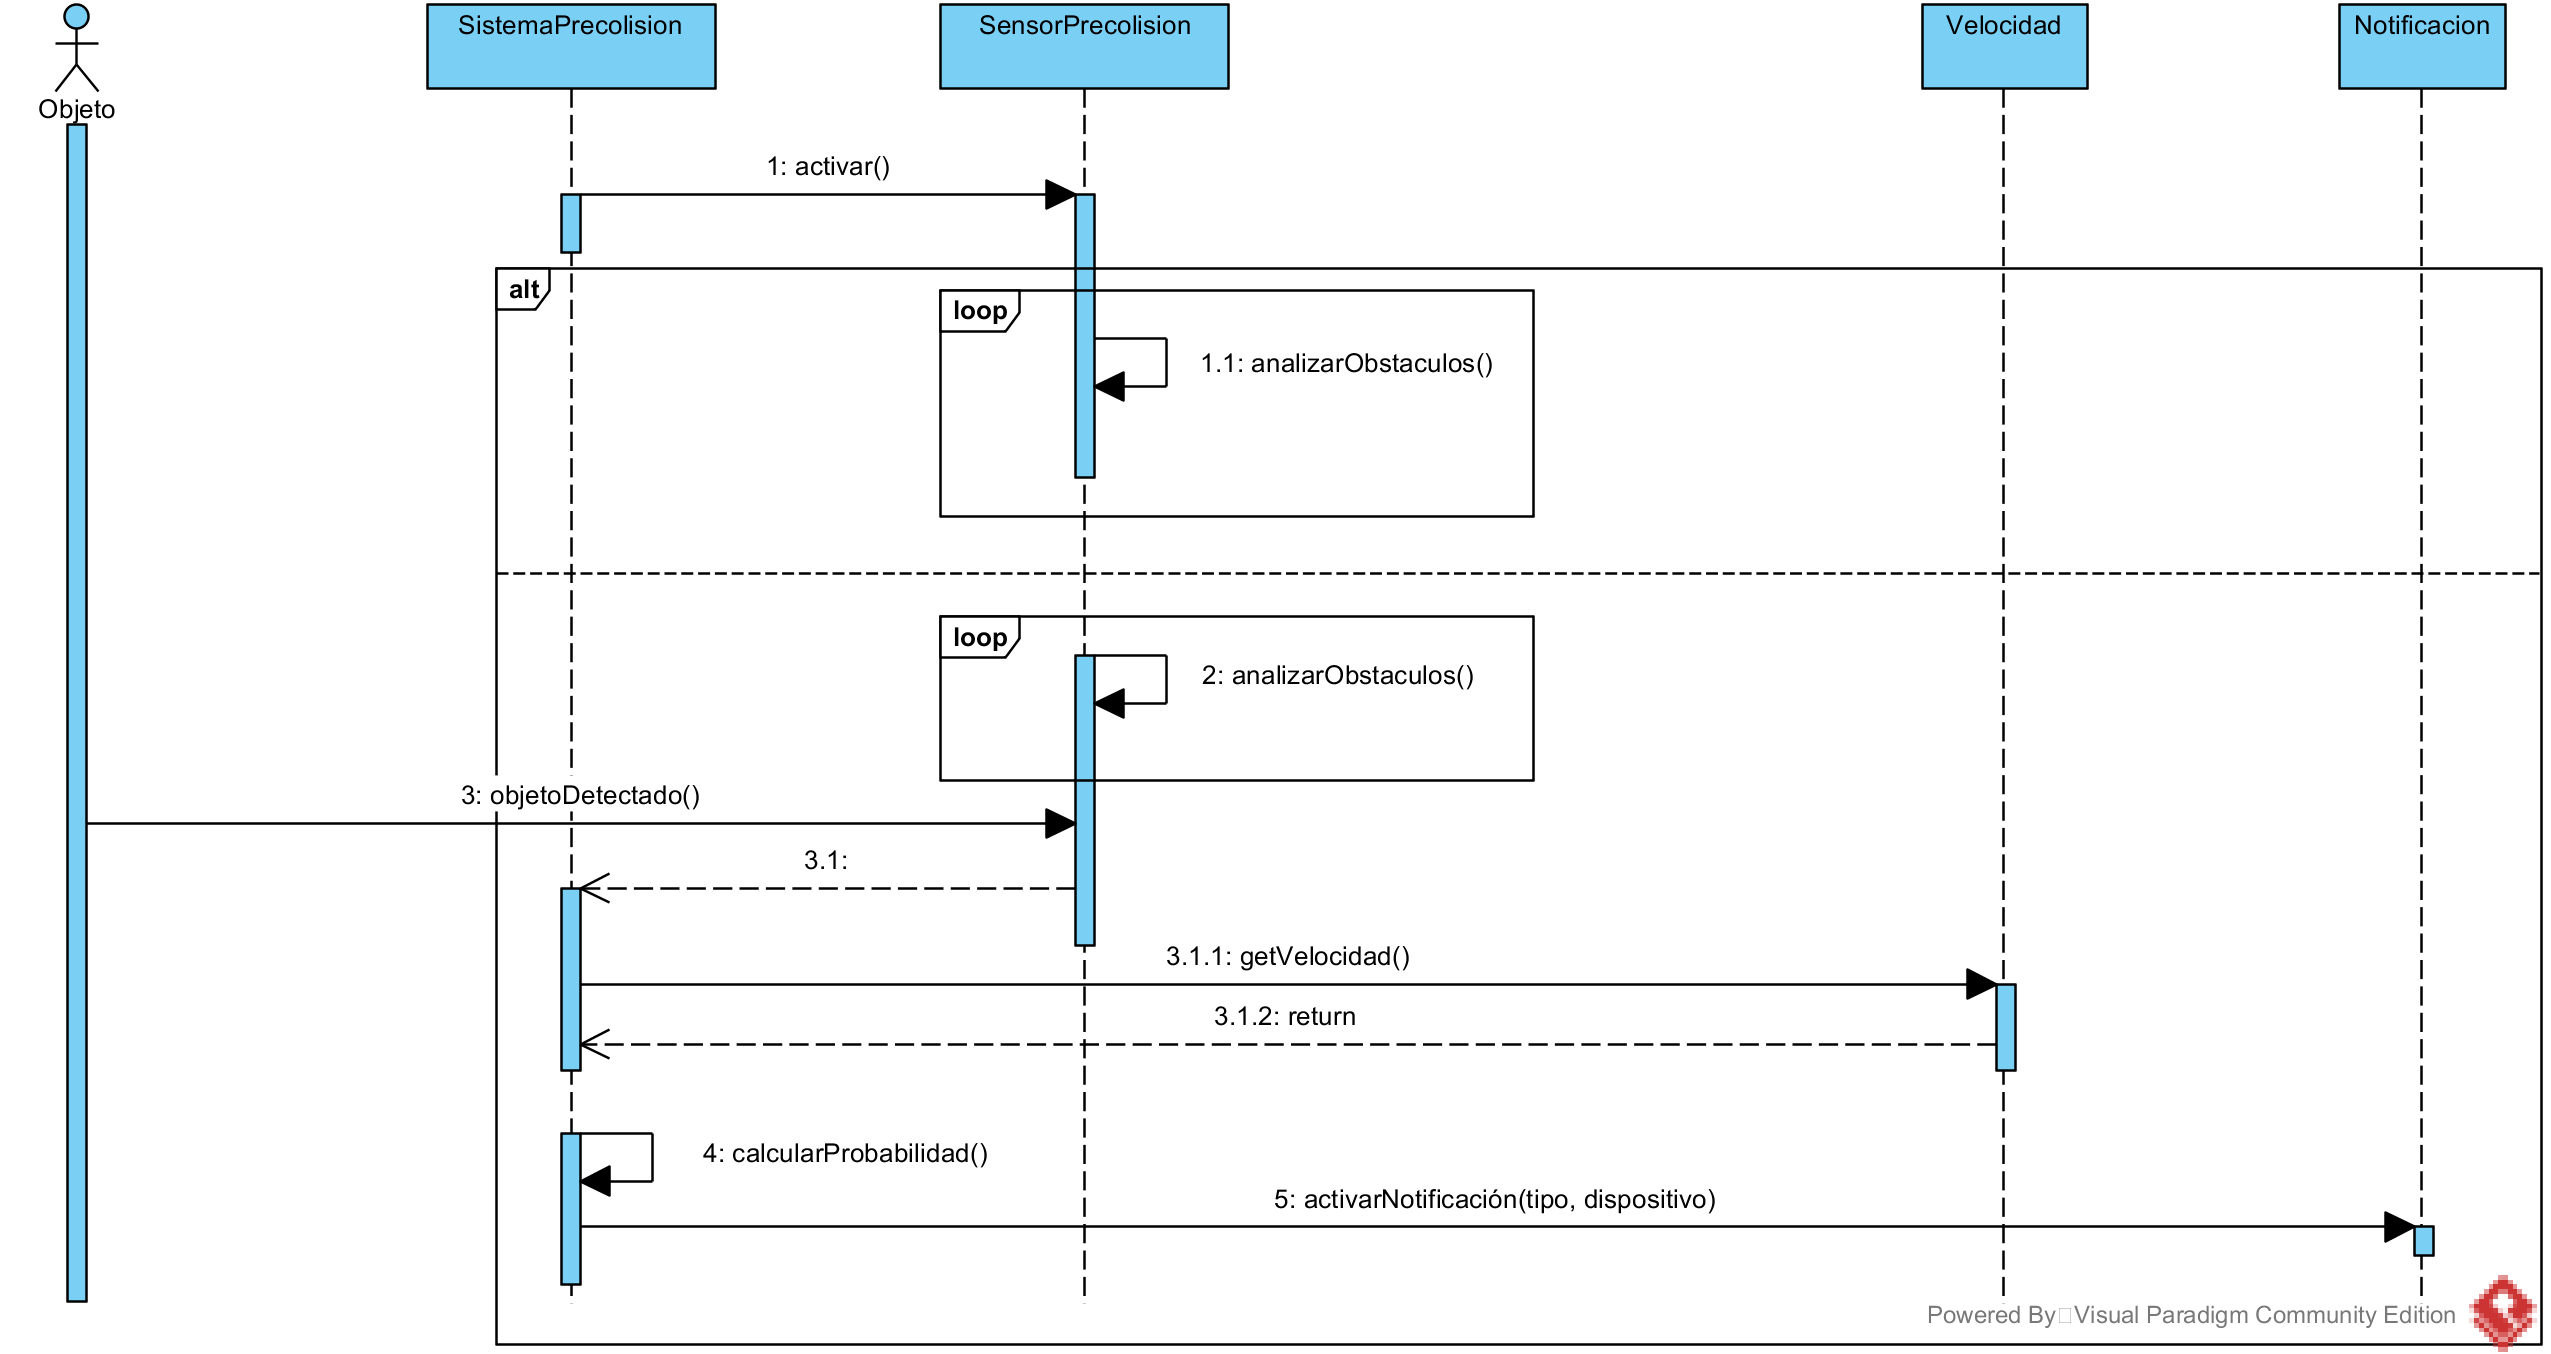
\includegraphics[width=0.8\textwidth]{./img/diagramas_de_secuencia/CDUE-11.png}
  \end{center}
  \caption{Diagrama de secuencia para el CDUE-11: \textit{Activar notificación por riesgo de colisión}}
  \label{img:not_riesgo_colision}
\end{figure}

\par El diagrama de secuencia de la figura \ref{img:reducir_velocidad} hace referencia al \nameref{tab:CDUE-13}. Este diagrama es muy similar los dos diagramas de secuencia explicados anteriormente, la diferencia radica en que después de calcular la probabilidad en el \textit{flujo de ejecución alternativo} se reduce la velocidad del vehículo.

\begin{figure}[h]
  \begin{center}
    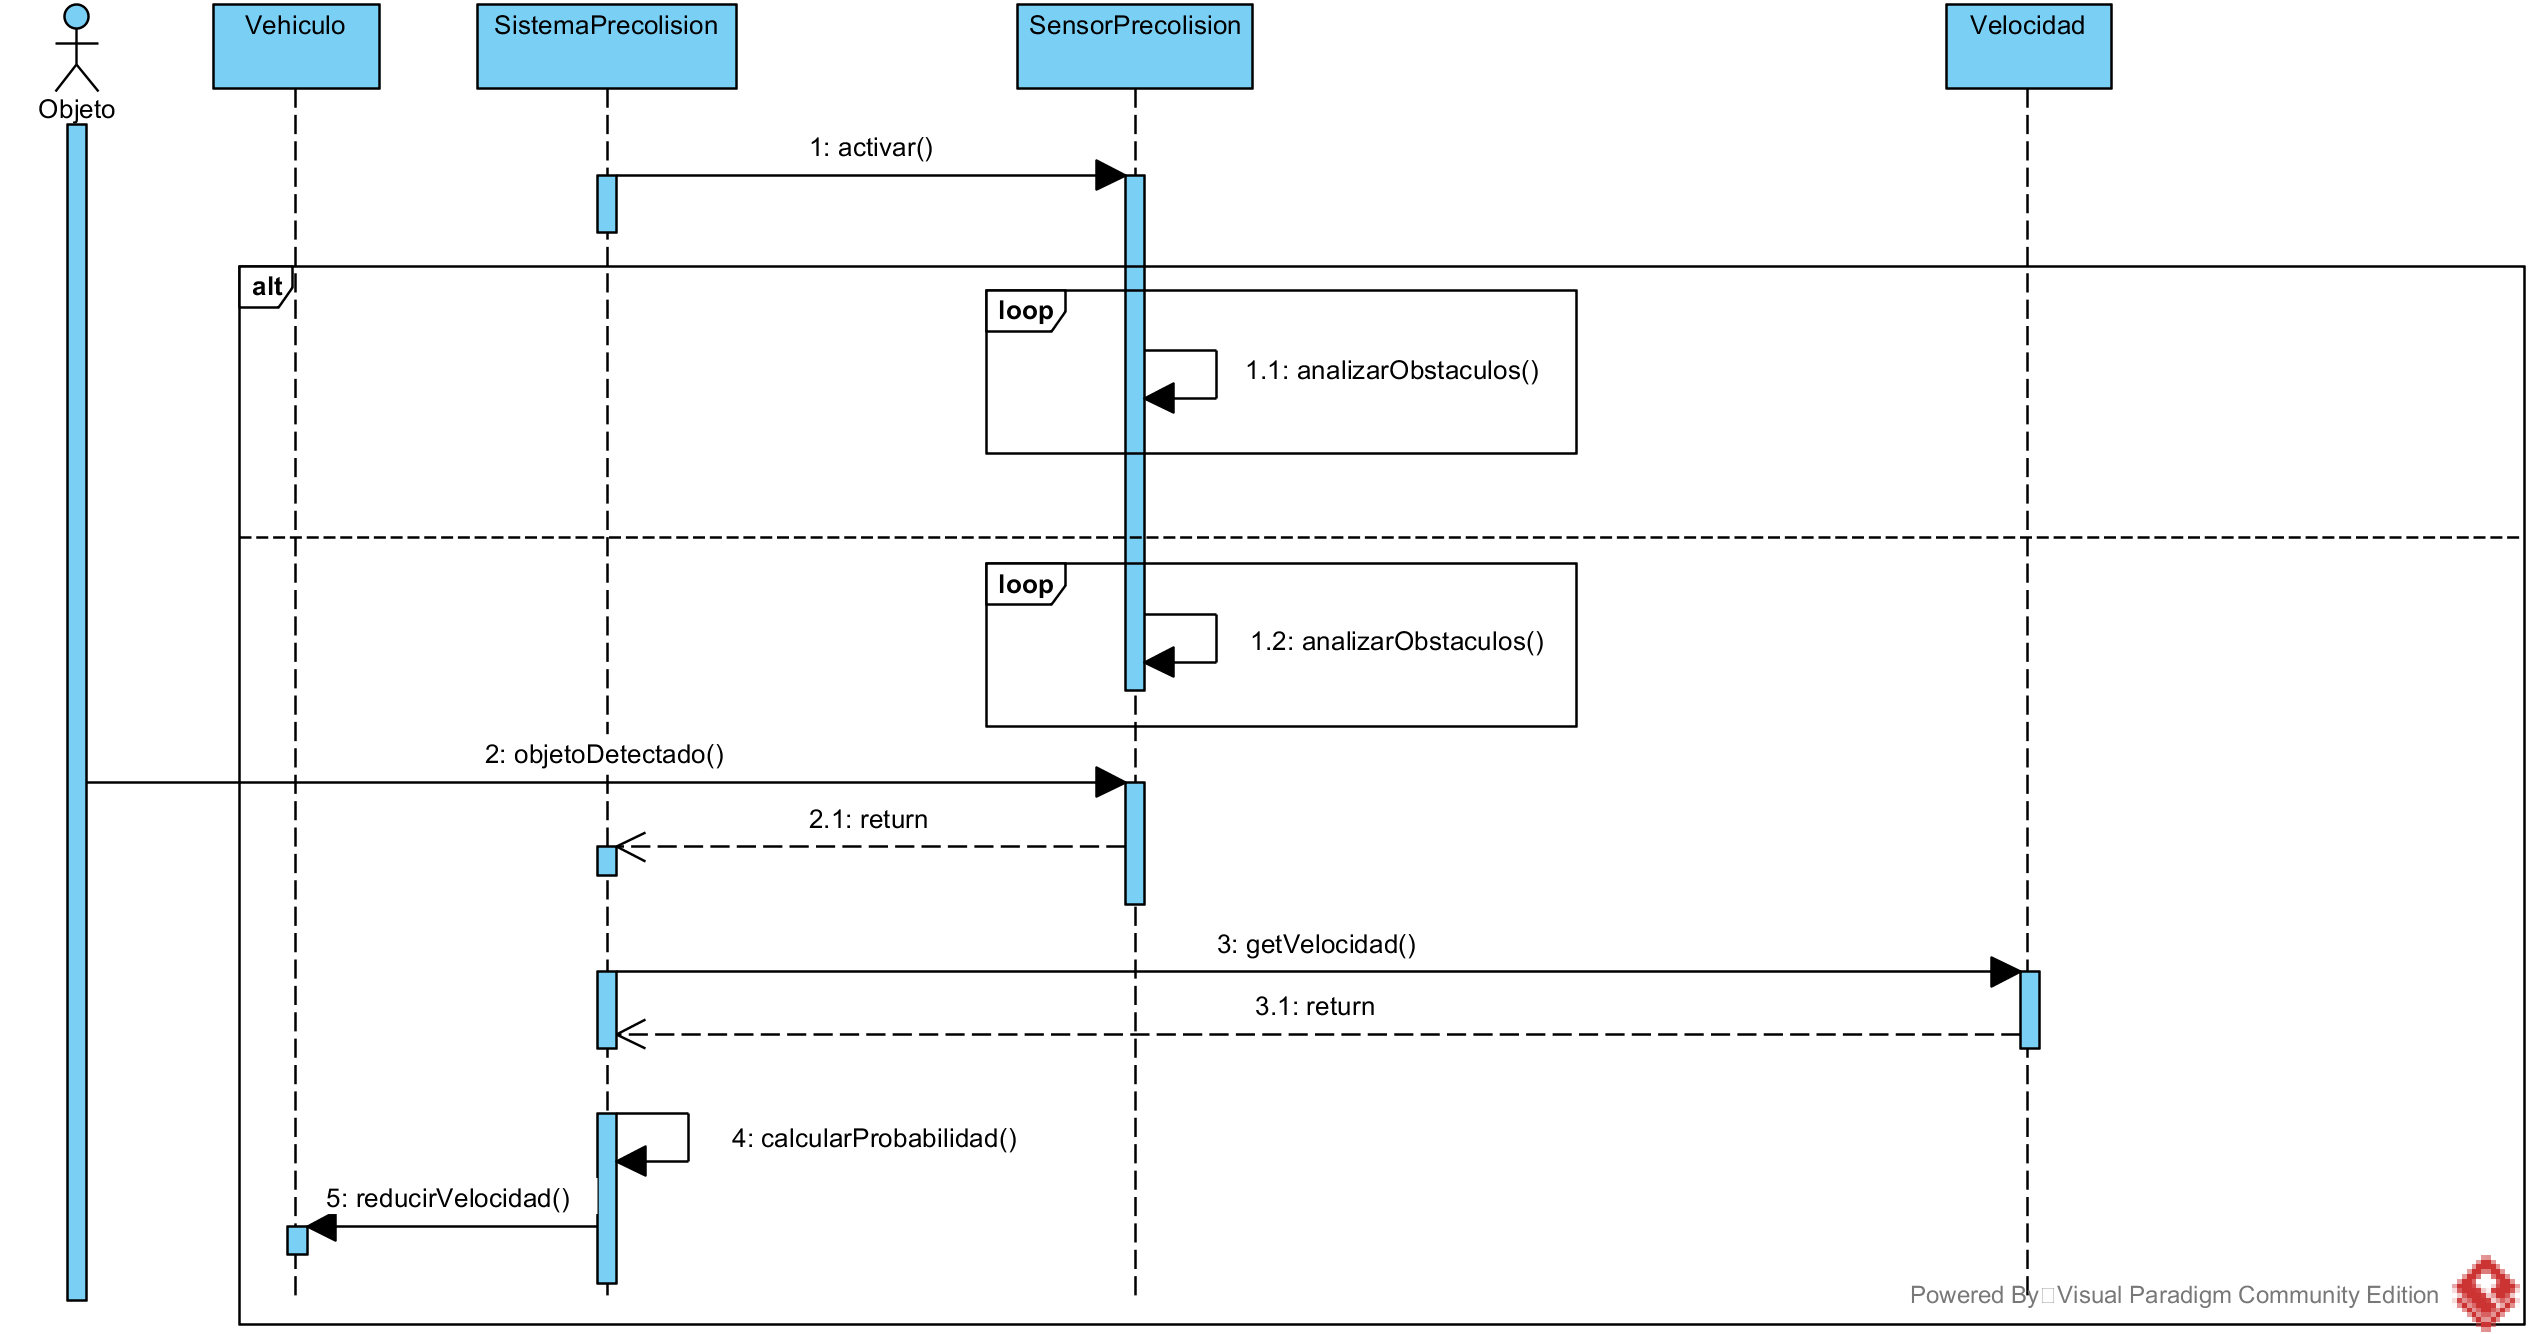
\includegraphics[width=0.8\textwidth]{./img/diagramas_de_secuencia/CDUE-13.png}
  \end{center}
  \caption{Diagrama de secuencia para el CDUE-13: \textit{Reducir velocidad}}
  \label{img:reducir_velocidad}
\end{figure}
